% ===== 02_model =====
\section{模型与阈值控制策略}
\label{sec:model}
\subsection{传播模型与基本假设}
人群分为易感者 $S$、隔离易感者 $S_q$、非隔离感染者 $I$、隔离感染者 $I_q$ 和康复者 $R$。接触率为 $c(t)$，一次接触的传播概率为 $\beta$，被有效追踪并隔离的接触者比例为 $q(t)$。其中，感染的被追踪者进入 $I_q$，未感染的被追踪者进入 $S_q$；未被追踪的感染者进入 $I$。两类感染者分别以速率 $\gamma$ 和 $\delta_q$ 移出。采用如下含接触追踪的 SIQR 型模型：
\begin{equation}
\begin{cases}
\dot S=-\dfrac{c(t)[\beta+(1-\beta)q(t)]}{N}SI,\\[.5em]
\dot I=\dfrac{\beta c(t)(1-q(t))}{N}SI-\gamma I,\\[.5em]
\dot S_q=\dfrac{(1-\beta)c(t)q(t)}{N}SI,\\[.5em]
\dot I_q=\dfrac{\beta c(t)q(t)}{N}SI-\delta_q I_q,\\[.5em]
\dot R=\gamma I+\delta_q I_q.
\end{cases}
\label{eq:model:full}
\end{equation}
\begin{figure}[htbp]
\centering
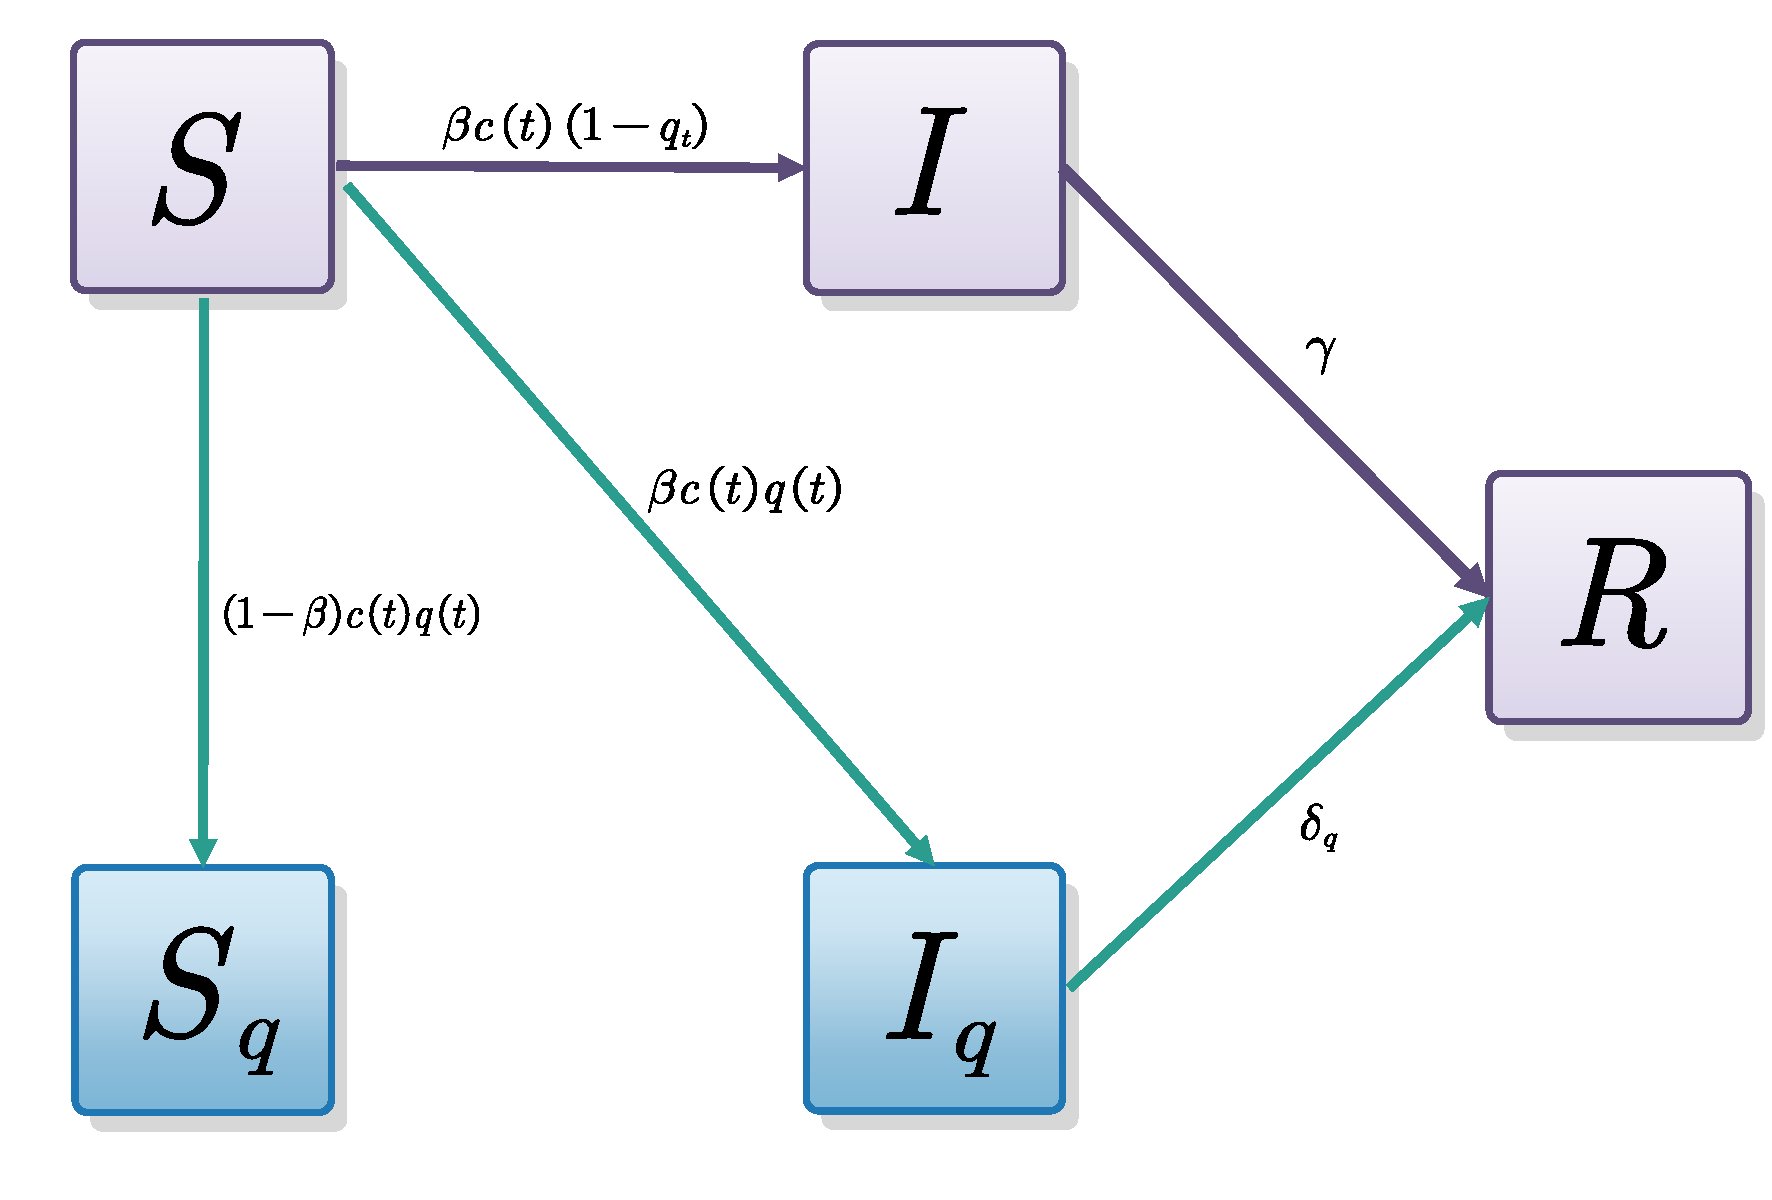
\includegraphics[width=0.7\textwidth]{figures/Fig1.pdf}
\caption{含接触追踪与隔离的 SIQR 型模型。$S,S_q,I,I_q,R$ 分别表示社区易感者、隔离易感者、非隔离感染者、隔离感染者和康复者。}
\label{fig:model_schematic}
\end{figure}

这一模型保留了文献\cite{Zhou2024SPCI}中社区传播与接触追踪的二维结构。以下假定 $N,c_0,\gamma,\delta_q>0$、$0<\beta\le1$、$0\le q_0<1$，初始仓室均非负且总和为 $N$，其中 $S_0,I_0>0$。人数以人为单位，$c,\gamma,\delta_q$ 的单位为时间的倒数，$\beta,q$ 为无量纲比例。文中沿用的“隔离率”指比例 $q$，不是检出感染者的连续时间风险率。

隔离者不参与社区传播，隔离易感者在研究时段内不返回 $S$；模型也不包括输入病例、出生和免疫丧失。在这些假设下，$S$ 的减少包含感染与未感染者隔离两部分，不能全部解释为感染后获得免疫。

\begin{proposition}
\label{prop:model:positive}
若 $c(t)\ge0$ 局部有界且可测，$q(t)\in[0,1]$ 可测，则式\eqref{eq:model:full}存在唯一全局绝对连续解，方程在几乎处处意义下成立。各仓室非负、总和恒为 $N$，且所有有限时刻均有 $S(t),I(t)>0$。
\end{proposition}
\begin{proof}
方程右端关于状态局部 Lipschitz，关于时间可测且在有界状态集上局部可积，故有唯一局部绝对连续解。前两式给出
\begin{align*}
S(t)&=S_0\exp\!\left[-\int_0^t\frac{c(s)[\beta+(1-\beta)q(s)]}{N}I(s)\,ds\right],\\
I(t)&=I_0\exp\!\left[\int_0^t\left(\frac{\beta c(s)(1-q(s))}{N}S(s)-\gamma\right)ds\right].
\end{align*}
隔离易感者的流入非负；隔离感染者由变参数公式保持非负；$\dot R\ge0$。五式相加得总人数守恒，因此所有分量有界，局部解可以延拓至任意有限时刻。上述指数表达式同时给出 $S,I$ 的严格正性。
\end{proof}

\subsection{感染上限、启动与退出条件}
\label{sec:model:strategy}
记 $\eta>0$ 为给定的社区非隔离感染人数上限，要求全过程满足 $I(t)\le\eta$，并记 $\theta=\eta/N$。该上限可参考医疗服务能力及防控目标选取\cite{Miclo2022ICU,Angulo2021}。本文将其作为外生参数，研究首次达到阈值后维持感染人数不变、并在满足退出条件时恢复常规控制的一类策略。

记常规控制为 $(c_0,q_0)$。当 $0<I_0<\eta$ 时，系统首先按常规控制演化。若常规感染峰值不超过 $\eta$，则无需为满足该上限加强干预；否则在感染人数首次上升至 $\eta$ 时启动，记该时刻为 $t_1$，并记 $S^*=S(t_1)$。本文规定控制期间满足
\begin{equation}
I(t)\equiv\eta,\qquad 0<c(t)\le c_0,\qquad q_0\le q(t)\le1,
\quad t_1\le t\le t_2.
\label{eq:model:plateau-requirement}
\end{equation}
这一阶段称为阈值控制期。由感染者方程，维持正的恒定感染人数要求
\begin{equation}
\frac{\beta c(t)(1-q(t))S(t)}{N}=\gamma.
\label{eq:model:balance}
\end{equation}
左端为单位非隔离感染者引起的新社区感染速率。固定 $c=c_0$ 时，该关系确定所需的隔离比例；允许 $c,q$ 同时调节时，它只规定两者必须共同满足的平衡。

常规控制下的临界易感者人数为
\begin{equation}
S_c=\frac{\gamma N}{\beta c_0(1-q_0)}.
\label{eq:model:Sc}
\end{equation}
本文规定 $t_2$ 为阈值控制期内首次达到 $S=S_c$ 的时刻，并在其后恢复 $(c_0,q_0)$。以下结果说明首次触发、维持阈值与上述退出条件各自的状态依据。

\Needspace{6\baselineskip}
\begin{proposition}
\label{prop:model:threshold-rationale}
设常规轨迹在有限时刻 $t_1$ 首次由下方到达 $I=\eta$，且 $S(t_1)=S^*>S_c$，则有以下结论。
\begin{enumerate}
\renewcommand{\labelenumi}{(\roman{enumi})}
\item 在首次加强干预之前采用 $(c_0,q_0)$ 的策略，若始终满足 $I\le\eta$，则首次加强干预的时刻不能晚于 $t_1$；常规轨迹在 $[0,t_1]$ 上满足该上限。
\item 在边界状态 $(S,\eta)$ 上，感染人数的瞬时导数非正当且仅当
\[
\frac{\beta c(1-q)S}{N}\le\gamma.
\]
若在一个时间区间内维持 $I=\eta$，则等号须几乎处处成立。
\item 从状态 $(S,\eta)$ 起恢复并保持 $(c_0,q_0)$，其后始终满足感染上限，当且仅当 $S\le S_c$。因此，沿任一从 $S^*>S_c$ 出发并持续维持 $I=\eta$ 的允许轨迹，首次达到 $S_c$ 是该轨迹上可以直接恢复常规控制的最早时刻。
\end{enumerate}
\end{proposition}
\begin{proof}
常规轨迹在首次到达时满足
\[
\dot I(t_1)=\eta\left[\frac{\beta c_0(1-q_0)S^*}{N}-\gamma\right]>0.
\]
若其后仍维持常规控制一段正时间，由连续性，感染人数会超过 $\eta$，故首次加强时刻不能晚于 $t_1$。在此之前不超过阈值则由首次到达的定义得到。

第二项直接由模型的感染者方程在 $I=\eta$ 时求得。对于有界可测时间控制，若 $I$ 在一个区间恒等于 $\eta$，则 $\dot I=0$ 几乎处处，故等号几乎处处成立。

恢复常规控制后有
\[
\dot I=\gamma I\left(\frac{S}{S_c}-1\right),\qquad
\dot S=-\frac{c_0[\beta+(1-\beta)q_0]}{N}SI<0.
\]
若恢复时 $S\le S_c$，此后 $S$ 严格下降，因而所有后续正时间均有 $\dot I<0$，感染人数不再超过 $\eta$。若恢复时 $S>S_c$，则恢复后的一个右邻域内有 $\dot I>0$，立即违反上限。阈值控制期内 $S$ 也严格下降，故沿该轨迹首次到达 $S_c$ 时即可恢复常规，而不能在此之前从阈值上直接退出。
\end{proof}

命题\ref{prop:model:threshold-rationale}中的最晚启动只相对于首次加强前未被改变的常规轨迹；最早退出只相对于已选定的恒定感染轨迹，不比较不同轨迹的退出时间。等式\eqref{eq:model:balance}表示感染增长恰好为零，既不唯一确定双控制分配，也不等于瞬时或累计成本最小。本文以这一规定过程作为研究对象，并不据此证明它在全部满足 $I\le\eta$ 的控制中最优。实施能力不足、观测误差或响应延迟存在时，可能需要提前干预或预留安全余量。

第\ref{sec:s1}--\ref{sec:s1:shape}节先固定 $c=c_0$，建立仅加强隔离的解析基准，并给出额外隔离能力上限下的实施判据；第\ref{sec:joint}节再允许两种控制同时变化，引入最低允许接触率 $c_{\min}$，考察两种能力限制下的可行分配。各策略在阈值控制期以外均采用相同的常规控制。第\ref{sec:joint}节的时间、感染和成本最优性均限定于相同进入与退出状态、始终保持 $I=\eta$ 的控制类，不比较提前干预、运行于 $I<\eta$ 或改变退出规则的方案。

\subsection{常规传播轨迹与触发条件}
$S,I$ 的方程不依赖其余仓室，因而启动与退出后的传播分析可归结为
\begin{equation}
\dot S=-\beta_1(t)SI,\qquad \dot I=\beta_2(t)SI-\gamma I.
\label{eq:model:reduced-si}
\end{equation}
其中
\begin{equation}
\beta_1(t)=\frac{c(t)[\beta+(1-\beta)q(t)]}{N},\qquad
\beta_2(t)=\frac{\beta c(t)(1-q(t))}{N}.
\label{eq:model:beta12-general}
\end{equation}
在常规阶段，记
\begin{equation}
\beta_1^0=\frac{c_0[\beta+q_0(1-\beta)]}{N},\quad
\beta_2^0=\frac{\beta c_0(1-q_0)}{N},\quad
\rho_1=\frac{\gamma}{\beta_1^0},\qquad
\frac{\beta_2^0}{\beta_1^0}=\frac{\rho_1}{S_c}.
\label{eq:model:beta12-baseline}
\end{equation}
消去时间或直接求导可得首次积分\cite{Zhou2024SPCI}
\begin{equation}
I(t)+\frac{\beta_2^0}{\beta_1^0}S(t)-\rho_1\ln S(t)=I_0+\frac{\beta_2^0}{\beta_1^0}S_0-\rho_1\ln S_0=:C_0,
\label{eq:model:first-integral}
\end{equation}
其中对数中的人数采用固定且统一的计数单位；后续计算均可写成人数比值。因此常规轨迹满足
\begin{equation}
I(S)=I_0+\frac{\beta_2^0}{\beta_1^0}(S_0-S)+\rho_1\ln\frac{S}{S_0}.
\label{eq:model:routine-orbit}
\end{equation}
当 $S_0\le S_c$ 时，所有 $t>0$ 均有 $I'(t)<0$，峰值为 $I_0$。当 $S_0>S_c$ 时，在 $S>S_c$ 的阶段有 $I\ge I_0$，从而 $\dot S\le-\beta_1^0 I_0S$，系统在有限时间到达 $S_c$。感染人数在该时刻由增转减，故常规峰值的完整表达为
\begin{equation}
I_{\max}^{no}=\begin{cases}
I_0,&S_0\le S_c,\\
I_0+\frac{\beta_2^0}{\beta_1^0}(S_0-S_c)+\rho_1\ln(S_c/S_0),&S_0>S_c.
\end{cases}
\label{eq:s1:Imax-no}
\end{equation}
以下关于正持续时间阈值控制的结果均在
\begin{equation}
S_0>S_c,\qquad 0<I_0<\eta<I_{\max}^{no}
\label{eq:model:trigger}
\end{equation}
下讨论。该条件保证常规传播会在达到峰值前触及感染上限。


